Ce programmame de test est assez simple, il effectue un saut de 4 instructions (@4 $\rightarrow$ @9), puis fini par déborder du programme et tombe sur de la mémoire où il n'y a que des \texttt{NOP}.

\begin{lstlisting}[language=VHDL]
--extrait du code de ROM.vhd

registres(0) <= X"000C0200"; --AFC R0,0x02 --2
registres(1) <= X"010B0000"; --COP R1,R0 -- 2
registres(2) <= X"02010001"; --ADD R2, R0, R1 R2<-R0+R1 -- 4
registres(3) <= X"04020002"; --MUL R4, R0, R2 R4<-R0*R2 -- 8
registres(4) <= X"00050400"; --JMP 0x4 (ip <= ip +4)
-- portion sautee
registres(5) <= X"060C2300"; --AFC R6,0x23
registres(6) <= X"070C7800"; --AFC R7,0x78
registres(7) <= X"090C9900"; --AFC R9,0x99
registres(8) <= X"020E0400"; --STORE 0x2, R4
-- fin de la portion sautee
registres(9) <= X"040D0200"; --LOAD R4, 0x2 -- 0 (valeur par defaut dans la RAM)
registres(11) <= X"0D070100"; --INF R13, R1 , R0 => false
registres(12) <= X"0E070004"; --INF R14, R0 , R4 => false
registres(13) <= X"0F090100"; --EQU R15, R1 , R0 => true
registres(14) <= X"0C090400"; --EQU R12, R4 , R0 => false
registres(15) <= X"0B080400"; --SUP R11, R4 , R0 => false
registres(16) <= X"0A080004"; --SUP R10, R0 , R4 => true
registres(17) <= X"000A0000"; --PRI R0 -- affiche 2
registres(18) <= X"0006FA0F"; --JMF R15, 0xFA
                              --(jump -6 impossible car R15 = true)
registres(19) <= X"0006010D"; --JMF R13, 0x01 (jump +1 avec R13 = false)
\end{lstlisting}

Une portion du chronogramme de ce test est présentée en figure \ref{simulation}. Le chronogramme présente le moment où le \texttt{JMP} est en train d'être exécuté. On voit bien la bulle générée due à la détection de l'aléa \texttt{jump\_JMP} ainsi que le saut de IP (\textit{Instruction Pointer}) de \texttt{0x06} à \texttt{0x09}.

\newpage

\begin{figure}[!H]
    \centering
    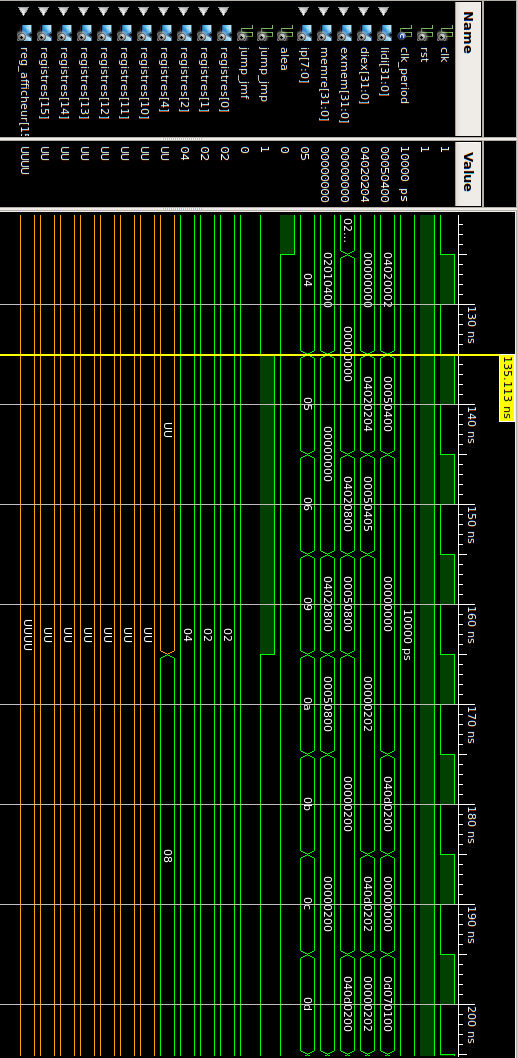
\includegraphics[scale=0.61]{simulation.png}
    \caption{Chronogramme de la simulation au moment du \texttt{JMP}}
    \label{simulation}
\end{figure}